\clearpage
\appendix
\tableofcontents

\section{Qualitative Results}

We present our qualitative results in the following website:
\href{https://diffmimic-demo-main-g7h0i8.streamlitapp.com/}{https://diffmimic-demo-main-g7h0i8.streamlitapp.com/}.

It contains the following qualitative results:
\begin{itemize}
    \item Back-Flip 20-second rollout.
    \item Cartwheel 20-second rollout.
    \item Crawl 20-second rollout.
    \item Dance 20-second rollout.
    \item Jog 20-second rollout.
    \item Jump 20-second rollout.
    \item Roll 20-second rollout.
    \item Side-Flip 20-second rollout.
    \item Spin-Kick 20-second rollout.
    \item Walk 20-second rollout.
    \item Zombie 20-second rollout.
    \item Back-Flip 20-second rollout, trained for 2.5 hours.
    \item Back-Flip single cycle rollout, trained for 10 minutes.
\end{itemize}

\section{Policy Network}
We use an MLP for the policy network. The network has two hidden layers with sizes 512 and 256. We use Swish~\citep{ramachandran2017searching} for the activation function.



\section{Hyper-parameters}
We use Adam optimizer~\citep{kingma2014adam} in training, with a learning rate of 3e-4 that linearly decreases with training iterations. We apply gradient clipping and set the maximum gradient norm to 0.3.  We set the batch size to the same as the number of parallel environments.

\textbf{Cyclic motions.} We set the maximum iterations to 5000. The number of environments is set to 200. 

\textbf{Acyclic motions.} We set the maximum iterations to 1000. The number of environments is set to 300.

\textbf{Expert Replay.} We run experiments with two error thresholds, 0.2 and 0.4, and report the better of the two.

\section{State and Action Space}
\textbf{Humanoid.}
We use 6d rotation representation~\citep{zhou2019continuity} in the state feature. The humanoid has an action size of 28 and a state feature size of 193.

\textbf{Humanoid with Sword and Shield.}
We set up the Sword and Shield character following ASE~\citep{peng2022ase}. Compared to the default humanoid, the new character has 3 additional DOF on the right hand. A sword is attached to its right hand and a shield is attached to its left lower arm. The character has an action size of 31. The state feature size is 208.

\clearpage

\section{Learning Curves}
\begin{table}[h!]
    \centering
    \begin{tabular}{ccc}
         \hspace{-10pt}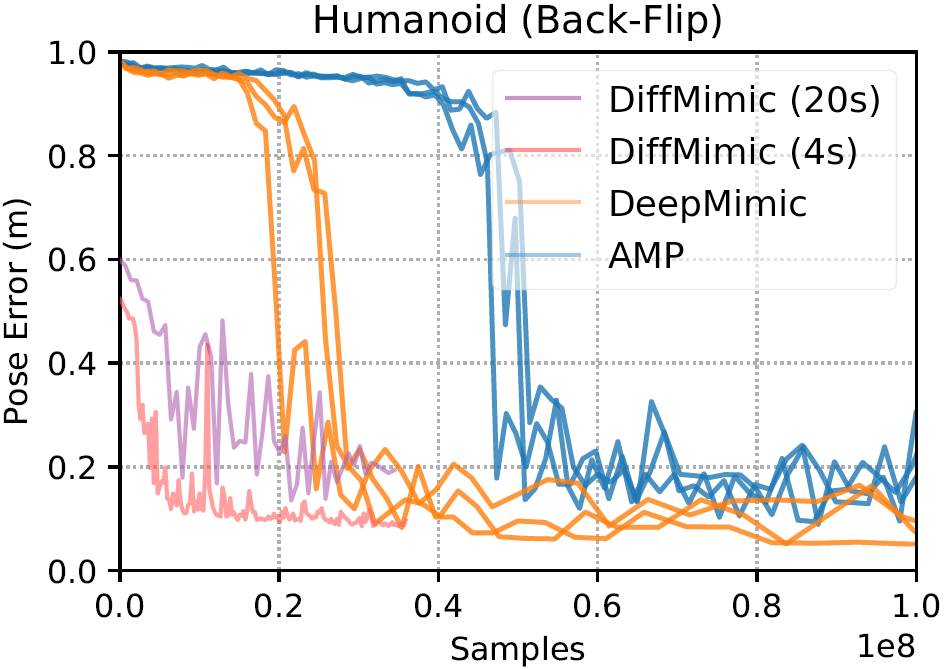
\includegraphics[width=0.31\textwidth]{figures/mixed_backflip_legend.png}
         &
         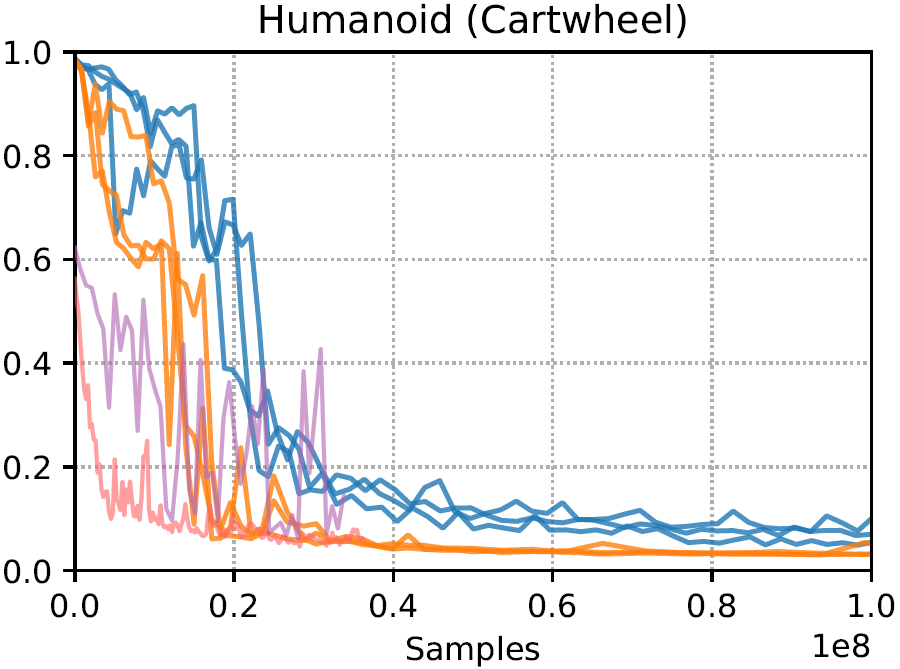
\includegraphics[width=0.31\textwidth]{figures/mixed_cartwheel.png}
         &
         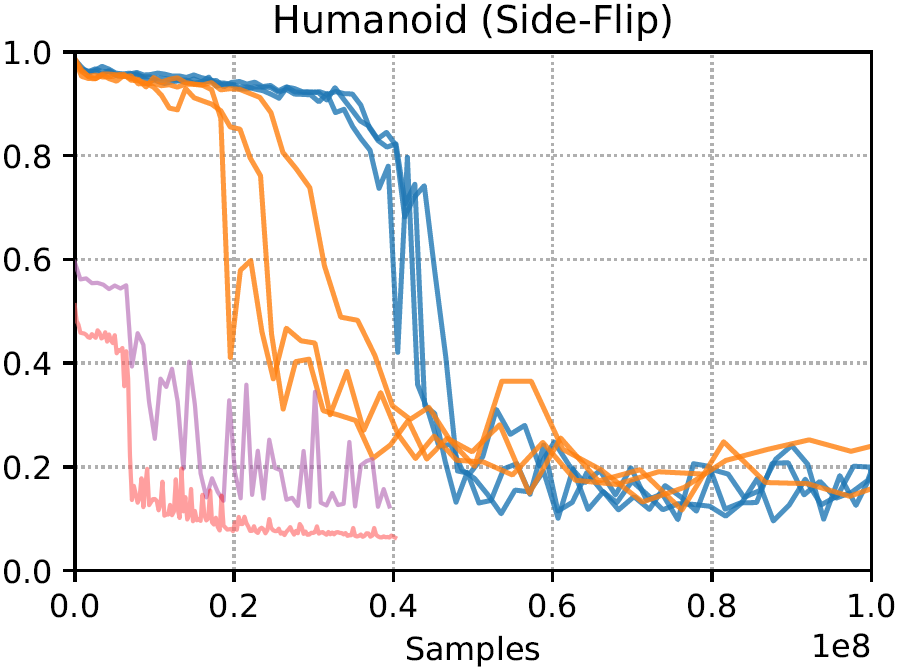
\includegraphics[width=0.31\textwidth]{figures/mixed_sideflip.png}
         \\
        \hspace{-10pt} 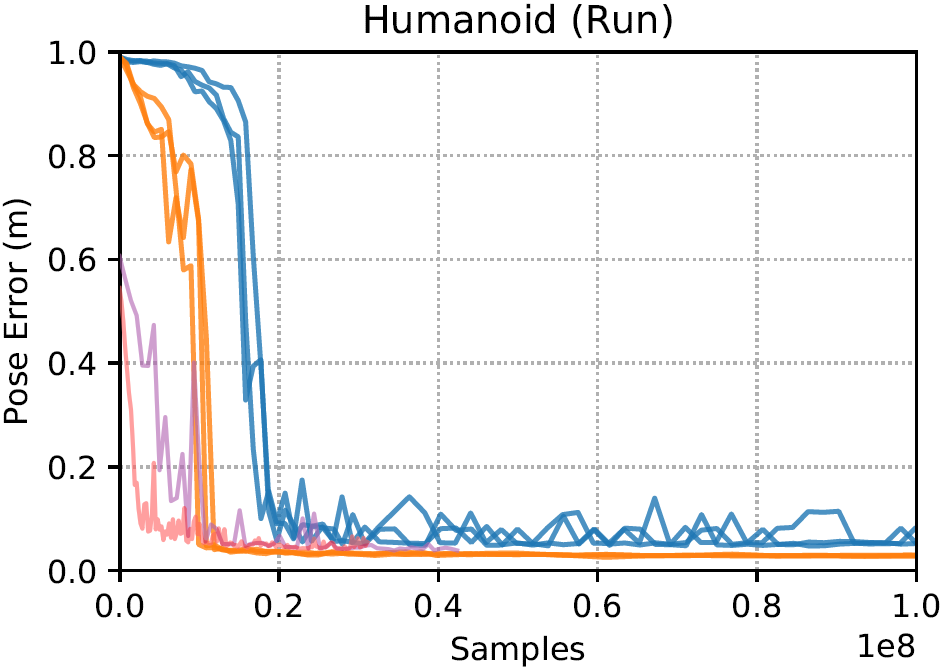
\includegraphics[width=0.31\textwidth]{figures/mixed_run.png}
         &
         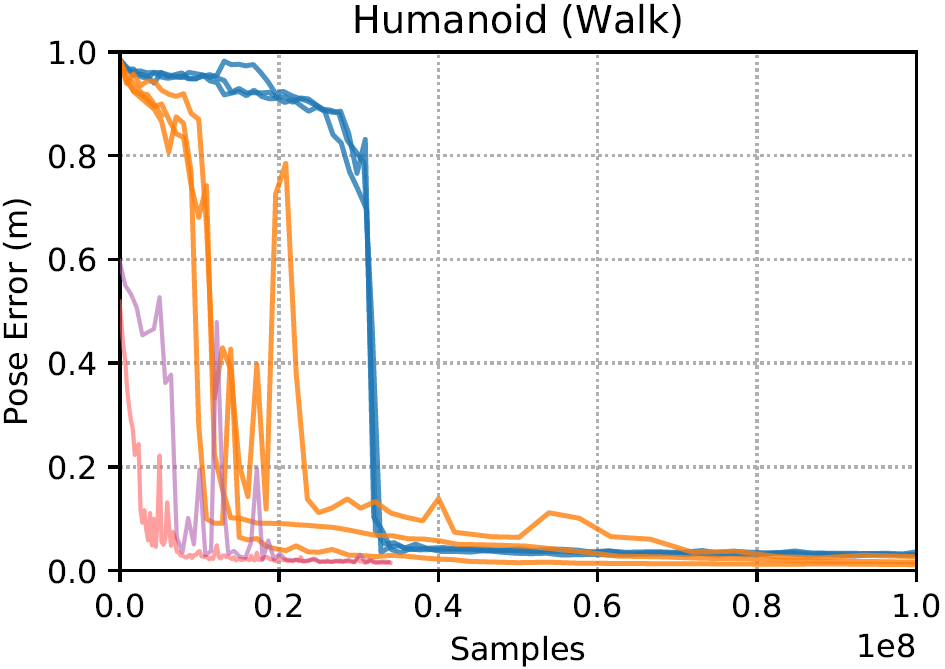
\includegraphics[width=0.31\textwidth]{figures/mixed_walk.png}
         &
         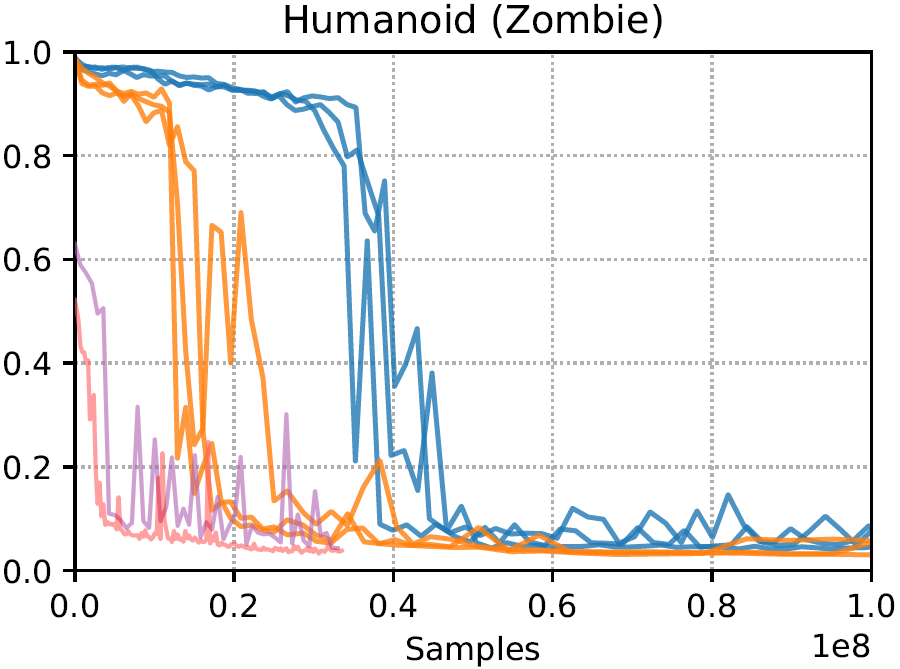
\includegraphics[width=0.31\textwidth]{figures/mixed_zombie.png}
         \\
         \hspace{-10pt}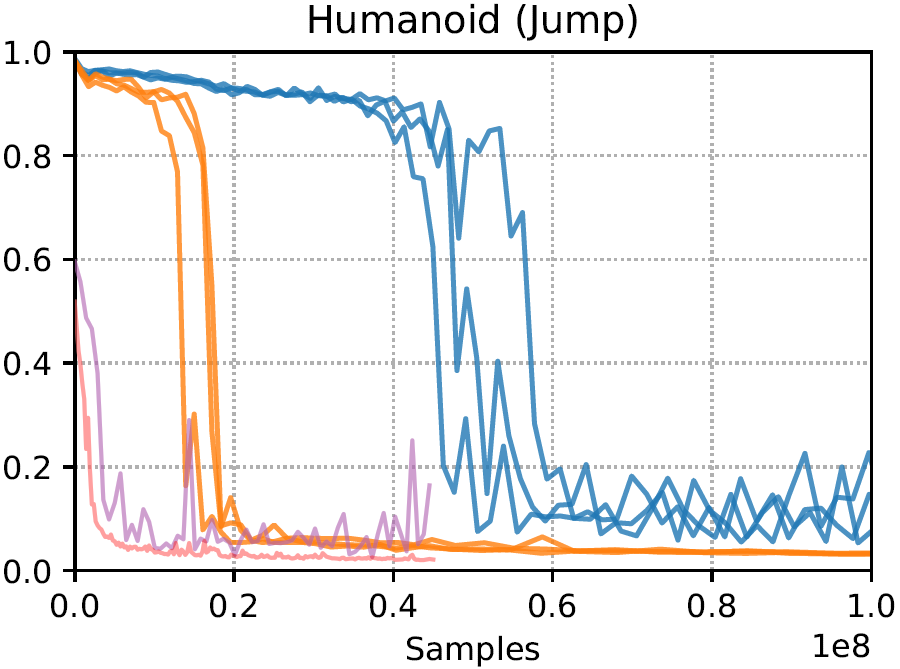
\includegraphics[width=0.31\textwidth]{figures/mixed_jump.png}
         &
         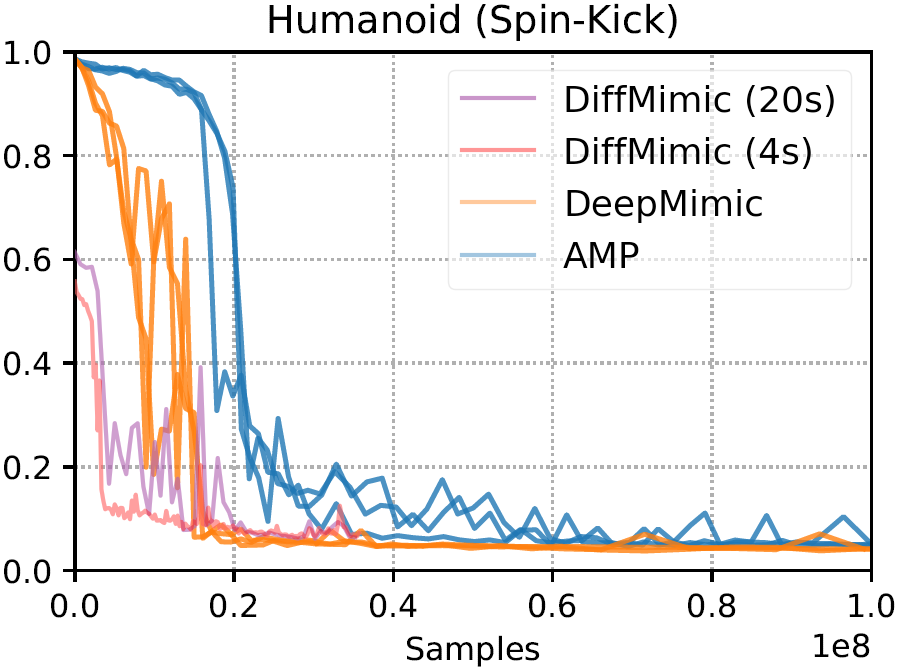
\includegraphics[width=0.31\textwidth]{figures/mixed_spinkick_legend.png}
         &
         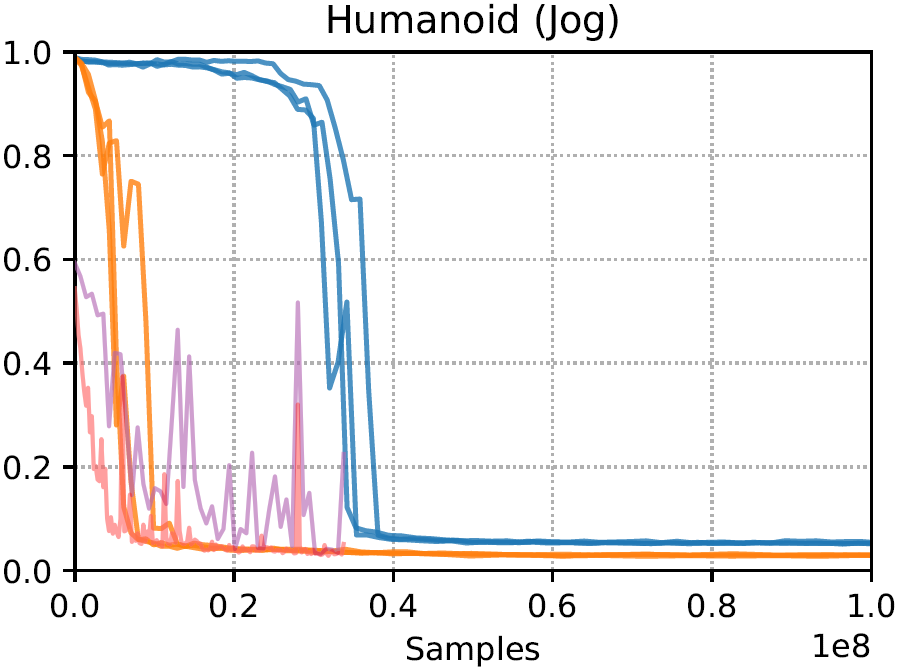
\includegraphics[width=0.31\textwidth]{figures/mixed_jog.png}
         \\
         \hspace{-10pt}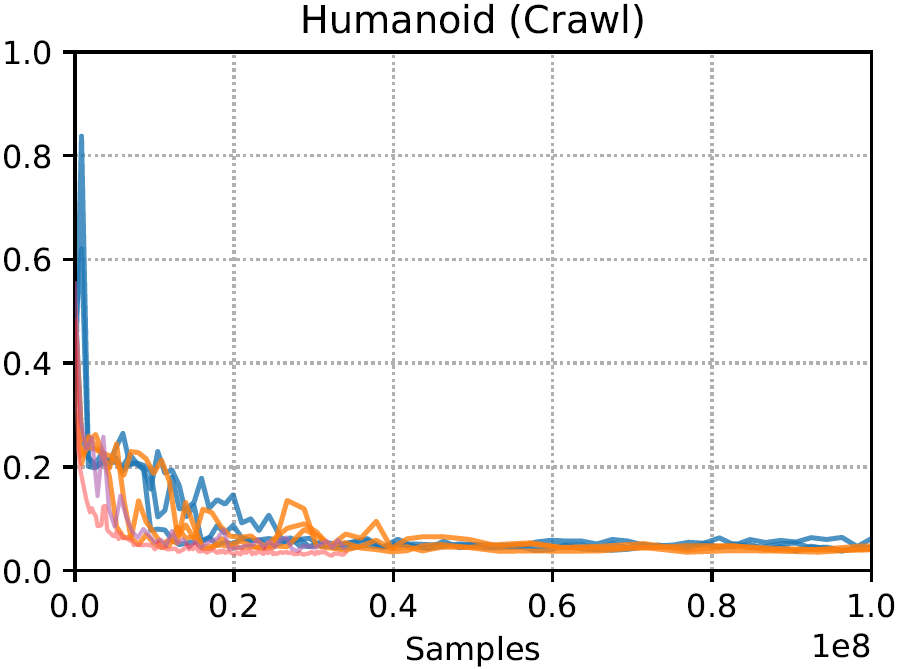
\includegraphics[width=0.31\textwidth]{figures/mixed_crawl.png}
         &
         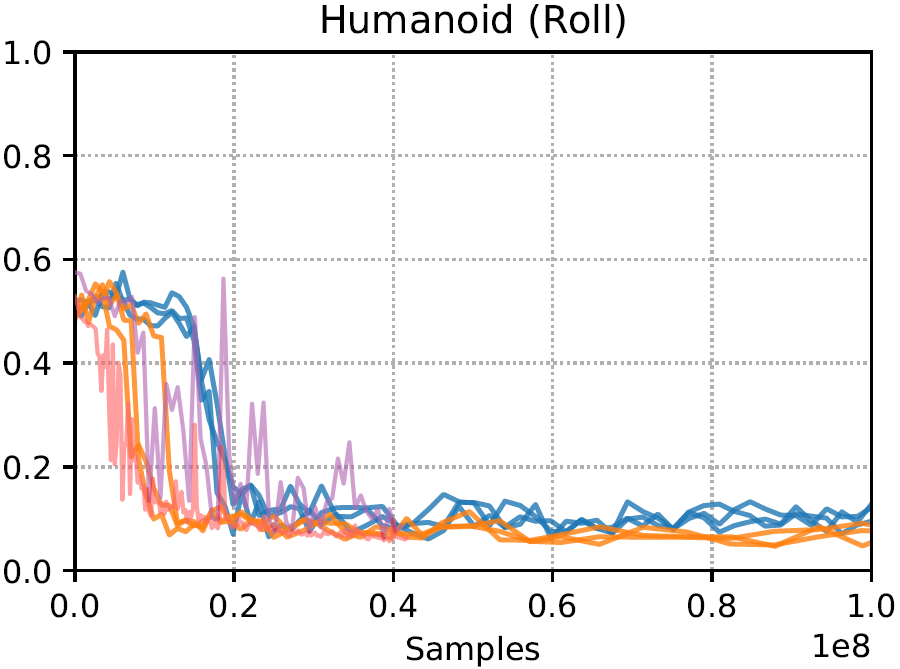
\includegraphics[width=0.31\textwidth]{figures/mixed_roll.png}
          &
         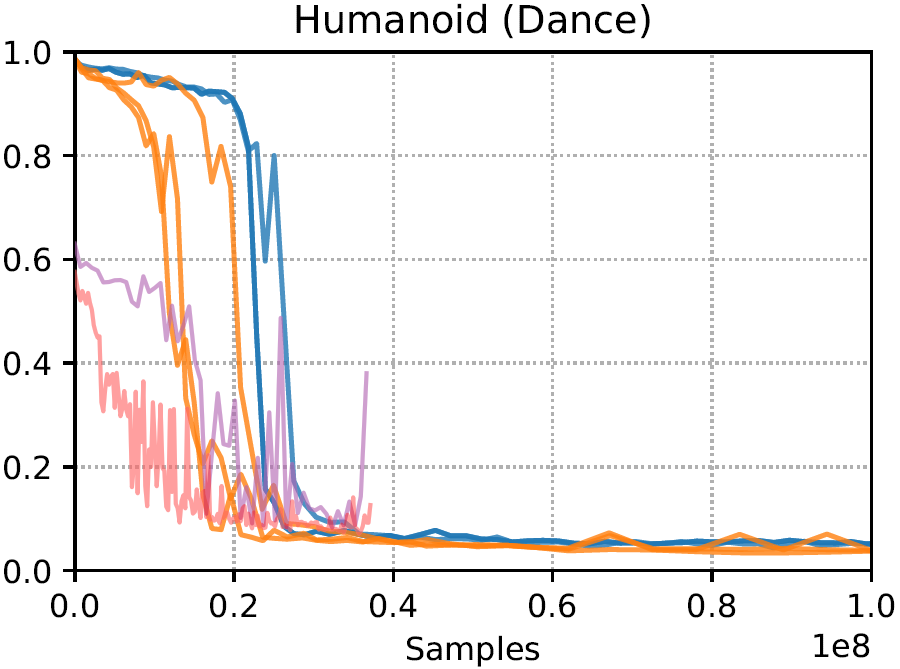
\includegraphics[width=0.31\textwidth]{figures/mixed_dance.png}
         
    \end{tabular}
    \captionof{figure}{Pose error versus the number of samples. DiffMimic (4s): rollout 4 seconds of Diffmimic for evaluation.  DiffMimic (20s): rollout 20 seconds of Diffmimic for evaluation.}
    \label{fig:imitate_one_full}
\end{table}




\clearpage

\section{{New Character}}
{We include Ant as a new character. We use the trajectory in ILD~\citep{chen2022imitation} as the reference motion, which is obtained from a PPO~\citep{schulman2017proximal} agent that learns to move forward as fast as possible. We achieve a 0.059 meter final pose error. We show the training curve in Figure~\ref{fig:ant}.} and the qualitative result on the  \href{https://diffmimic-demo-main-g7h0i8.streamlit.app/}{demo website} under the tab "New Character".
\begin{figure}[h]
    \centering
    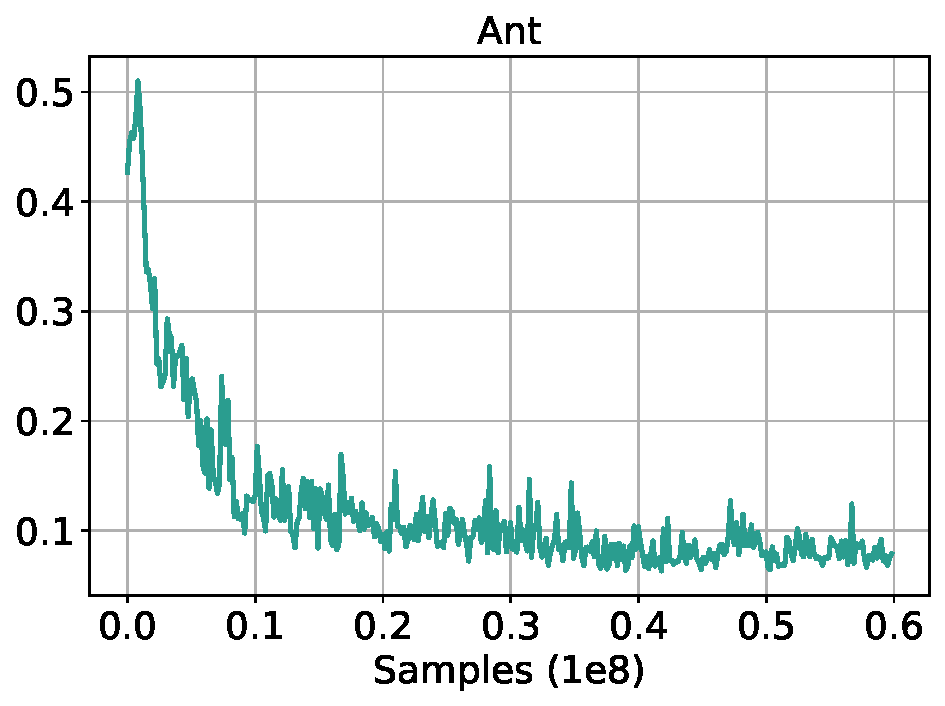
\includegraphics[width=.4\textwidth]{figures/Ant.pdf}
    \captionof{figure}{Pose error versus the number of samples for the new character, Ant.}
    \label{fig:ant}
\end{figure}


\section{{New Skill}}
{We run DiffMimic on a new skill, \emph{360-degree Jump}, from the CMU Mocap Dataset (motion sequence CMU\_075\_09). The skill has been reported to be challenging for a RL-based method CoMic~\citep{hasenclever2020comic} in a recent dataset paper~\citep{wagener2022mocapact}. DiffMimic is able to spin in the air and achieve a 0.020 meter final pose error. We show the training curve in Figure~\ref{fig:360-degree Jump}} and the qualitative result on the \href{https://diffmimic-demo-main-g7h0i8.streamlit.app/}{demo website} under the tab "New Skill".


\begin{figure}[h]
    \centering
    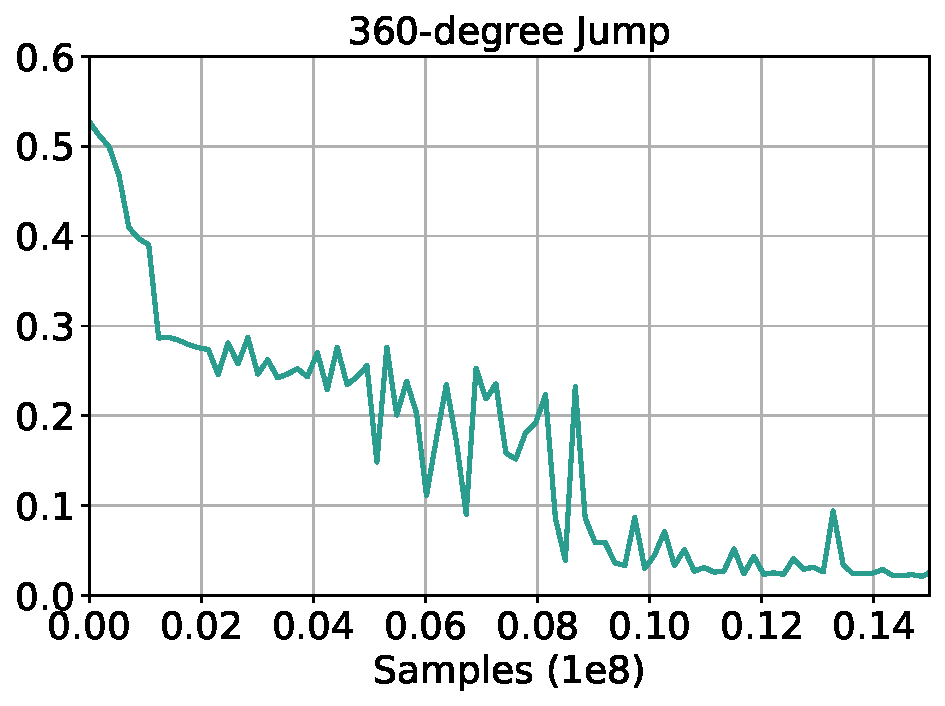
\includegraphics[width=.4\textwidth]{figures/rebuttal/360-degree-Jump.pdf}
    \captionof{figure}{Pose error versus the number of samples for the new skill, \emph{360-degree Jump}.}
    \label{fig:360-degree Jump}
\end{figure}


\section{{New Training Strategy}}
We additionally include the Reference State Initialization (RSI) technique~\citep{peng2018deepmimic} into the DiffMimic training. RSI starts the training rollout from a random reference frame instead of the first reference frame. We observe a substantial empirical improvement after employing the new training strategy. The samples required are consistently around 90\% less than DeepMimic~\citep{peng2018deepmimic} as shown in \autoref{tab: rsi_sampleeff}. The final pose error has also been slightly improved as shown in \autoref{tab: rsi_poseerror}. We show the qualitative results on the \href{https://diffmimic-demo-main-g7h0i8.streamlit.app/}{demo website} under the tab "New Training". Notably, using RSI alone or RSI+Early Termination (ET)~\citep{peng2018deepmimic} does not converge as shown in Figure~\ref{tab:rsi-curve}.
\begin{table}[h]
\caption{ {Number of samples required to roll out 20 seconds without falling in $(10^6)$ with Reference State Initialization (RSI)~\citep{peng2018deepmimic}. Percentage: change in the fraction of the DeepMimic samples.}}
\label{tab: rsi_sampleeff}
\begin{center}
\begin{tabular}{lccccc}
\toprule
Motion & $\textrm{T}_\textrm{cycle}$(s) &  DeepMimic  & Spacetime Bound  & Ours & Ours w/ RSI\\
\midrule

Back-Flip & 1.75 & 31.18 & 41.20 \plusstyle{+32.1\%} & 14.88 \minusstyle{-52.2\%} & 3.82 \minusstyle{-87.7\%} \\
Cartwheel & 2.72  & 30.45 & 17.35 \minusstyle{-43.0\%} & 13.92 \minusstyle{-54.2\%}& 4.72 \minusstyle{-84.5\%}\\
Walk & 1.25  & 23.80 & 4.08 \minusstyle{-79.5\%} & 7.92 \minusstyle{-66.7\%} & 1.55 \minusstyle{-93.5\%}\\
Run & 0.80  & 19.31 & 4.11 \minusstyle{-78.7\%} & 8.16 \minusstyle{-57.7\%} & 1.41 \minusstyle{-92.7\%}\\
Jump & 1.77  & 25.65 & 41.63 \plusstyle{+77.8\%} & 5.28 \minusstyle{-79.4\%}  & 2.12 \minusstyle{-91.7\%}\\
Dance & 1.62  & 24.59 & 10.00 \minusstyle{-59.3\%} & 16.56 \minusstyle{-32.6\%} & 2.19 \minusstyle{-91.1\%}\\

\bottomrule
\end{tabular}
\end{center}
\end{table}
\begin{table}[h]
\caption{{Pose error comparison in meters.  $\textrm{T}_\textrm{cycle}$ is the length of the reference motion for a single cycle. The error is averaged on 32 rollout episodes with a maximum length of 20 seconds. The result of Ours+RSI is obtained without DTW.}}
\fontsize{8}{9}\selectfont
\label{tab: rsi_poseerror}
\begin{center}
\begin{tabular}{lcccccc}
\toprule
Motion & $\textrm{T}_\textrm{cycle}$(s) &  DeepMimic & AMP & Ours  & Ours w/o DTW  & Ours w/ RSI\\
\midrule
Back-Flip & 1.75 & 0.076 $\pm$ 0.021 & 0.150 $\pm$ 0.028 & 0.097 $\pm$ 0.001 & 0.105 $\pm$ 0.022 &0.058$\pm$ 0.015\\
Cartwheel & 2.72 & 0.039 $\pm$ 0.011 & 0.067 $\pm$ 0.014 & 0.040 $\pm$ 0.007 & 0.040 $\pm$ 0.007  &0.027$\pm$ 0.002 \\
Crawl & 2.93 & 0.044 $\pm$ 0.001 & 0.049 $\pm$ 0.007 & 0.037 $\pm$ 0.001 & 0.037 $\pm$ 0.001 &0.035$\pm$ 0.003\\
Dance & 1.62 & 0.038 $\pm$ 0.001 & 0.055 $\pm$ 0.015 & 0.070 $\pm$ 0.003 & 0.072 $\pm$ 0.014 & 0.042$\pm$ 0.001\\
Jog & 0.83 & 0.029 $\pm$ 0.001 & 0.056 $\pm$ 0.001 & 0.031 $\pm$ 0.002 & 0.031 $\pm$ 0.002 &0.012$\pm$ 0.000\\
Jump & 1.77 & 0.033 $\pm$ 0.001 & 0.083 $\pm$ 0.022 & 0.025 $\pm$ 0.000 & 0.031 $\pm$ 0.002 & 0.015$\pm$ 0.000\\
Roll & 2.02 & 0.072 $\pm$ 0.018 & 0.088 $\pm$ 0.008 & 0.061 $\pm$ 0.007 & 0.083 $\pm$ 0.001 & 0.046$\pm$ 0.005\\
Run & 0.80 & 0.028 $\pm$ 0.002 & 0.075 $\pm$ 0.015 & 0.039 $\pm$ 0.000 & 0.046 $\pm$ 0.000 & 0.019$\pm$ 0.000\\
Side-Flip & 2.44 & 0.191 $\pm$ 0.043 & 0.124 $\pm$ 0.012 & 0.069 $\pm$ 0.001 & 0.121 $\pm$ 0.009 & 0.035$\pm$ 0.001\\
Spin-Kick & 1.28 & 0.042 $\pm$ 0.001 & 0.058 $\pm$ 0.012 & 0.056 $\pm$ 0.000 & 0.056 $\pm$ 0.000& 0.036$\pm$ 0.000\\
Walk & 1.30 & 0.018 $\pm$ 0.005 & 0.030 $\pm$ 0.001 &  0.017 $\pm$ 0.000 &  0.017 $\pm$ 0.000 &0.012$\pm$ 0.000\\
Zombie & 1.68 & 0.049 $\pm$ 0.013 & 0.058 $\pm$ 0.014 & 0.037 $\pm$ 0.002 & 0.037 $\pm$ 0.002 & 0.033$\pm$ 0.009\\
\bottomrule
\end{tabular}
\end{center}
\end{table}

\begin{table}[]
    \centering
    \begin{tabular}{cccc}
    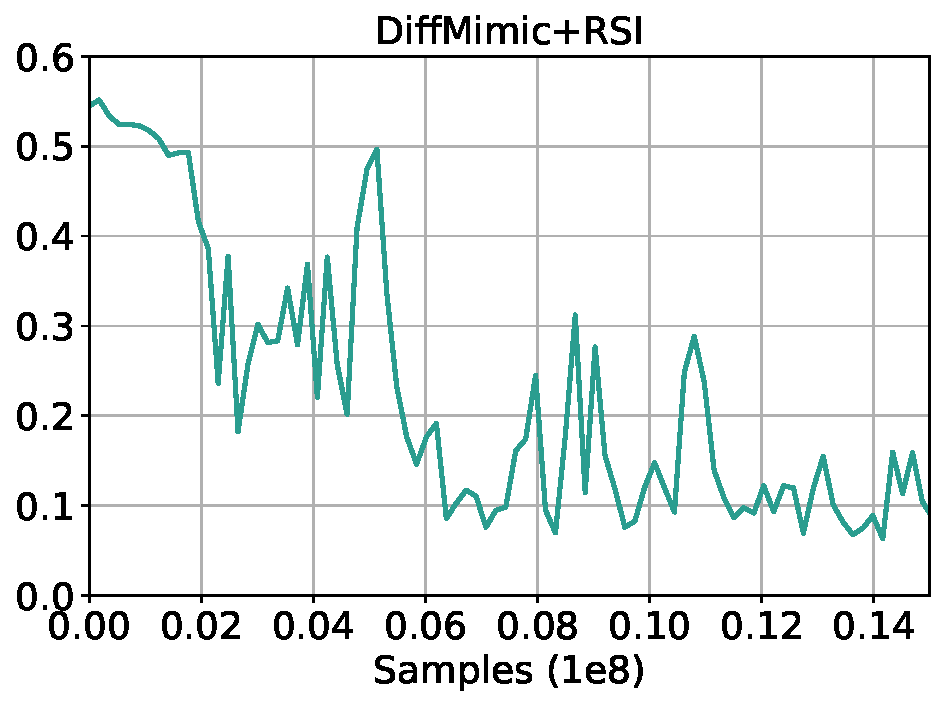
\includegraphics[width=0.3\textwidth]{figures/rebuttal/DiffMimic_RSI.pdf}&
    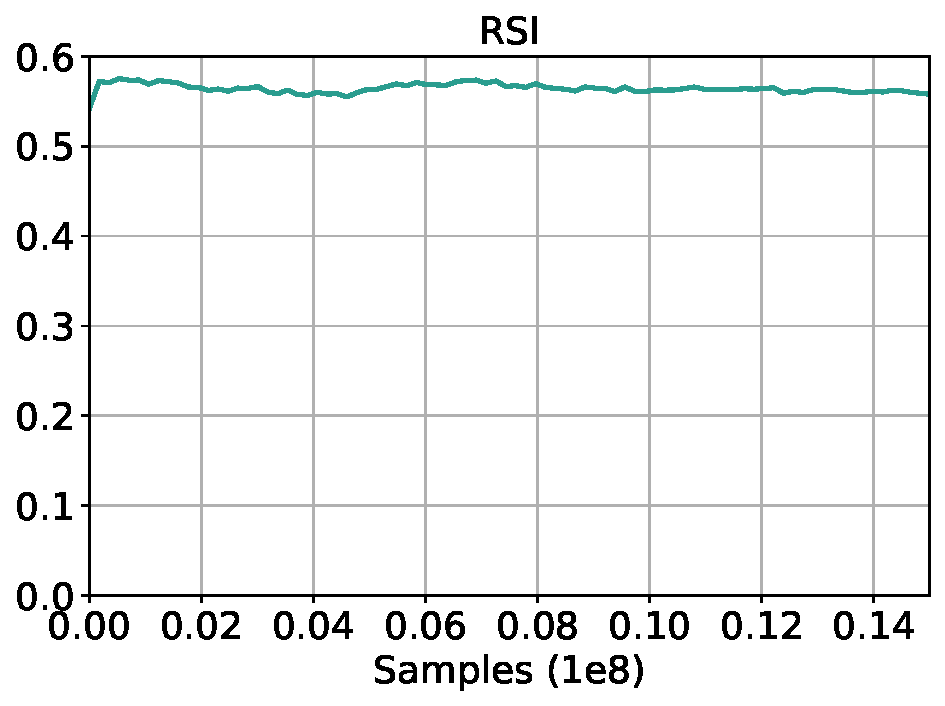
\includegraphics[width=0.3\textwidth]{figures/rebuttal/RSI.pdf}&
    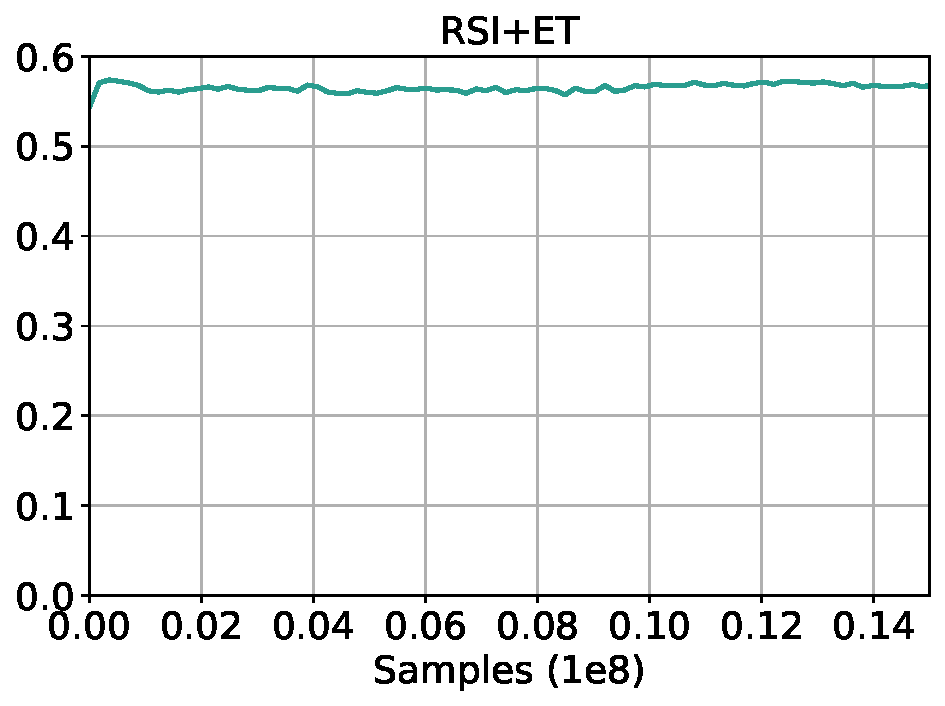
\includegraphics[width=0.3\textwidth]{figures/rebuttal/RSI_ET.pdf}&
    \\
    (a)
    &
    (b)
    &
    (c)
    \end{tabular}
    \captionof{figure}{{Pose error versus the number of samples on \emph{Back-Flip} using (a) DiffMimic+RSI (b) standalone RSI (c) RSI+ET.}
    }
    \label{tab:rsi-curve}
\end{table}

\section{Analysis on Robustness}
We further evaluate DiffMimic's robustness to external forces. A force is applied to the pelvis of the character halfway through a motion cycle for 0.2 seconds, and we measure the maximum forwards and sideways push each policy can tolerate before falling. DiffMimic achieves comparable robustness to DeepMimic. We show the results in Table~ \ref{tab:robustness} and the qualitative results on the \href{https://diffmimic-demo-main-g7h0i8.streamlit.app/}{demo website} under the tab "Robustness".
\begin{table}[h]
\caption{ {Maximum forwards and sideways push each policy can tolerate before falling. Each push is applied halfway through a motion cycle to the character’s pelvis for 0.2s. F: Forwards push. S: Sideways push. The unit is in Newton.}}
\label{tab:robustness}
\begin{center}
\begin{tabular}{l|rr|rr}
\toprule
Motion & 
DeepMimic (F)& 
Ours (F)&
DeepMimic (S) &
Ours (S)\\
\midrule
Back-Flip & 440 & \textbf{750} & 100 & \textbf{310} \\
Cartwheel & 200 & \textbf{350} & 470 & \textbf{690} \\
Run & \textbf{720} & 500 & \textbf{300} & 270 \\
Spin-Kick & \textbf{690} & 630 & 600 & \textbf{730} \\
Walk & 240 & \textbf{250} & \textbf{300} & 220 \\
\bottomrule
\end{tabular}
\end{center}
\end{table}

\section{Analysis on Sensitivity}
DiffMimic with inaccurate estimates of physical parameters. Briefly speaking, DiffMimic is able to learn the control policy well even though the friction coefficient deviates from the original parameters. We show the results in Table~\ref{tab:friction} and the qualitative results on the \href{https://diffmimic-demo-main-g7h0i8.streamlit.app/}{demo website} under the tab "Sensitivity".
\begin{table}[!h]
\caption{ {Sensitivity to the friction coefficient $\mu$, a system parameter. The evaluation is conducted on Zombie Walk, a motion heavily impacted by the friction coefficient. $\mu=1.0$ is the standard setting, we additionally evaluate when $\mu=0.8$ and $\mu=1.2$.}}
\label{tab:friction}
\begin{center}
\begin{tabular}{l|r}
\toprule
Friction &
Pose Error (m)\\
\midrule
$\mu$=0.8 &
0.047$\pm$ 0.009 \\
$\mu$=1.0 & 
0.032$\pm$ 0.009 \\
$\mu$=1.2 & 
0.028$\pm$ 0.007 \\
\bottomrule
\end{tabular}
\end{center}
\end{table}


\section{{Analysis on Motion Quality}}
Motion quality can be severely affected by a small number of large error poses, which can not be reflected by the existing average pose error metric. We propose a Pose Absurdity metric to quantify large-error poses. L2@0.01, 0.05, and 0.1 measure the average L2 pose error on the worst 1\%, 5\%, and 10\% frames
respectively. Full Horizon Gradient, Demonstration Replay (Random) ratio $\lambda$, and Demonstration Replay (Threshold) threshold $\gamma$ are studied. Demonstration Replay (Threshold) outperforms other baselines by a large margin. We show the results in Table~ \ref{tab:metric}

\begin{table}[h]
\caption{ {Ablation experiment on Full Horizon Gradient, Demonstration Replay (Random) ratio $\lambda$, and Demonstration Replay (Threshold) threshold $\gamma$ with the new Pose Absurdity metric on \emph{Back-Flip}.  L2@0.01, 0.05 and 0.1 measure the average L2 pose error on the worst 1\%, 5\% and 10\% frames respectively. Demonstration Replay (Threshold) significantly improves on the Pose Absurdity metric.}}
\label{tab:metric}
\begin{center}
\begin{tabular}{l|rrr}
\toprule
Method & L2@0.01 & L2@0.05 & L2@0.1 \\
\midrule
full horizon & 0.357 & 0.343 & 0.323 \\
\midrule
$\lambda$ = 0.01 & 0.379 & 0.341 & 0.318 \\
$\lambda$ = 0.05 & 0.195 & 0.177 & 0.135 \\
$\lambda$ = 0.10 & 0.359 & 0.332 & 0.262 \\
\midrule
$\gamma$ = 0.1 & 0.111 & 0.107 & 0.095 \\
$\gamma$ = 0.2 & 0.113 & 0.107 & \textbf{0.093} \\
$\gamma$ = 0.4 & \textbf{0.110} & \textbf{0.103} & 0.095 \\
\bottomrule
\end{tabular}
\end{center}
\end{table}







\section{Swording Character}
\begin{figure}[h]
    \centering
    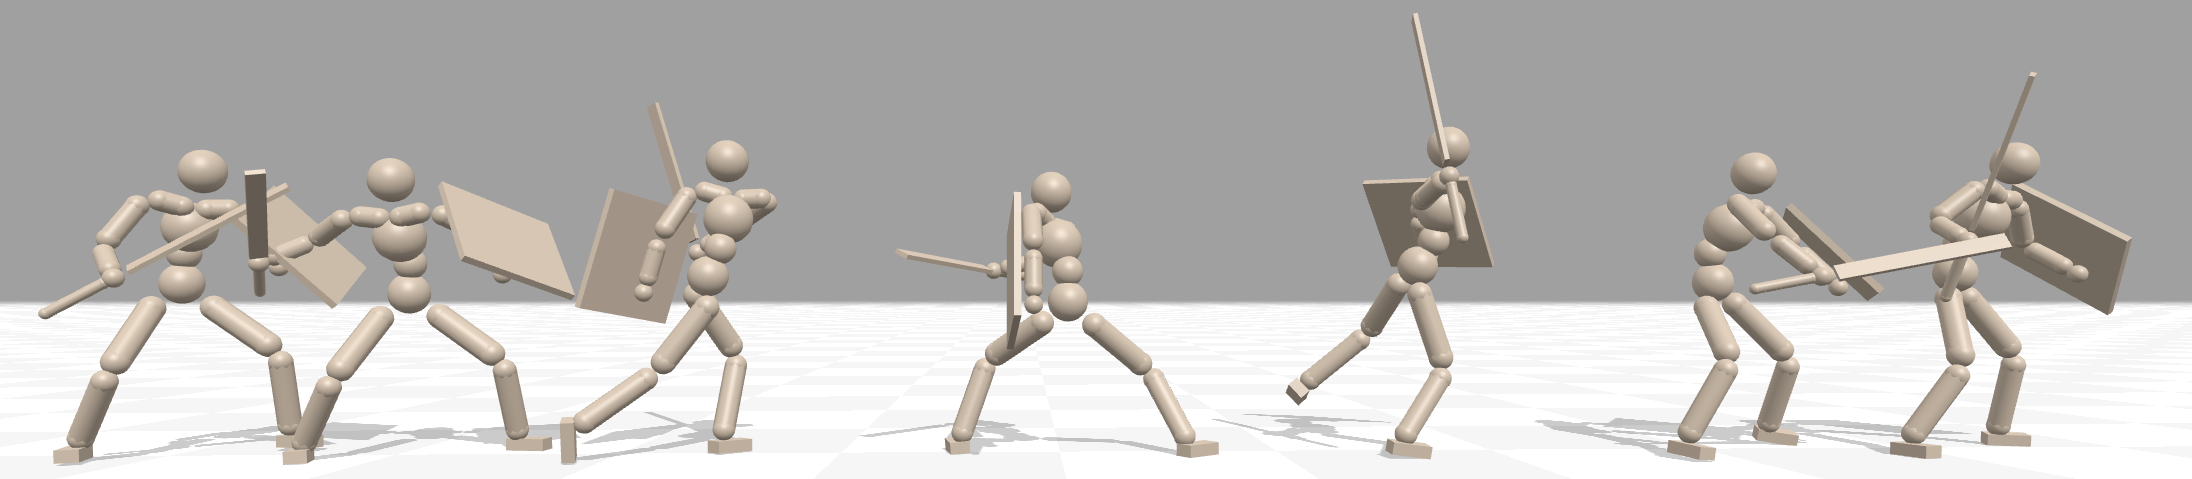
\includegraphics[width=\textwidth]{figures/qp/sword_shield.png}
    \caption{Character performing attack move with a sword and a shield. The reference motion clip is from Reallusion~\citep{Reallusion}}
    \vspace{-20pt}
    \label{fig:sword}
\end{figure}







